\newpage
\section{方法}
\subsection{使用器具}
今回の実験で使用した器具を\wtab{kigu}に示す.\\
なお,実験指導書ではソフトが``NI LabVIEW2015(32ビット)''と記載されていたが,使用したPCにインストールされていたものは``NI LabVIEW2019SPI(32ビット)''であった.

\begin{table}[hbtp]
  \centering
  \caption{実験装置}
  \label{tab:kigu}
  \scalebox{0.75}{
  \begin{tabular}{cccccc}
    \hline
    機器名&製造元&型番&シリアル番号&数量\,個\\
    \hline
    PC&iiyama&NK50SZ&NKNK50SZ0000K00088&1\\
    組み込みデバイス&NATIONAL INSTRUMENTS&myRIO-1900&308778E&1\\
    ブレッドボードアクセサリ&DEGILENT&MXP Breadboard for NI myRIO&D535760&1\\
    ソフトウェア&NATIONAL INSTRUMENTS&LabVIEW&LabVIEW2019 19.0.H3(32-bit)&1\\
    \hline
  \end{tabular}
  }
\end{table}

\subsection{実験手順}
プログラムの実行が速く,目視による確認が難しい場合,``ハイライトモード''を有効にすると実行過程がゆっくり表示されるようになる.
また以下では,基本的なLabVIEWの操作方法については述べない.
\subsection{実習2-1}
\subsubsection{導通確認}
\begin{enumerate}[a)]
	\item MXPブレッドボードアクセサリとジャンパーワイヤーを使って\wfig{2.12}のように回路を構築.その後,アクセサリボードをmyRIOのAポートに接続.
	\item ブロックダイアグラムで,``Analog Input''(Channel欄には,``A/AI 0(pin3)''を選択)を配置し,同右コネクタ(A/AI 0 pin3)に,``表示器''を作成.
	\item 上の計測プログラムを実行.
	\item \wfig{2.12}において``接続先を変更する''と記載されている端子をGND, 3.3\,\rm{V}, 5\,\rm{V}それぞれに接続し,値が正しく変化することを確認した.
\end{enumerate}
\begin{figure}
\centering
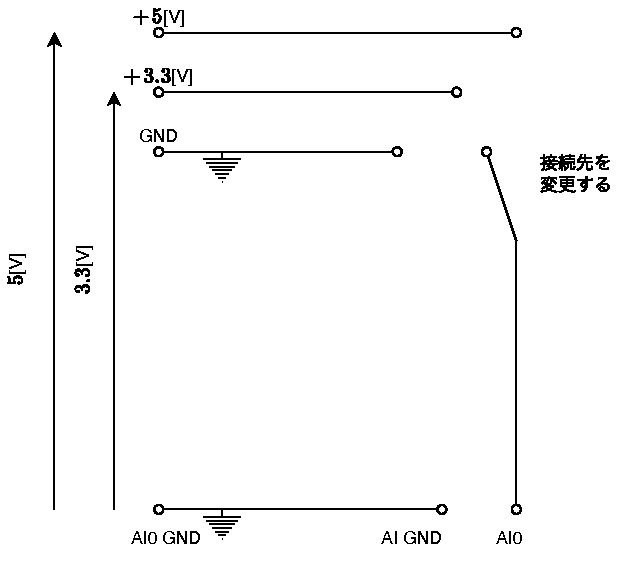
\includegraphics[scale=0.7]{/Users/ohyamasan/Downloads/TMCIT-Report/EE_Measurement/fig/100-volt.pdf}
\caption{定電圧計測回路}
\label{fig:2.12}
\end{figure}

\subsubsection{``For ループ''}
\begin{enumerate}[a)]
	\item 上で作成した``Analog Input''ブロックと表示器とを``Forループ''で囲むように配置し,``i''に表示器を作成.
	\item ``For ループ''のコネクタ``N''に定数を作成し5を代入.
	\item 上記プログラムを実行し正しく動作していることを確認した.
	\item ``Analog Input''の右コネクタ(A/AI 0 pin3)と``For ループ''の右端枠に接続し,コネクタに表示器を作成.(名前が``配列''に変更される)
	\item 作成したプログラムを実行し.``配列''(フロントパネル上の)に表示器(A/AI0)に表示された値が表示されることを確認した.
\end{enumerate}

\subsubsection{``配列連結追加''}
\begin{enumerate}[a)]
	\item 上の``For ループ''プログラムに``配列連結追加''ブロックを配置し,同左コネクタをカウンタ変数``i''に接続.
	\item ``配列連結追加''の左コネクタに``入力を追加''を選択し,数値入力用の左コネクタが2つになることを確認した.
	\item ``配列連結追加''ブロックの左コネクタを``Analog Input''の右コネクタ(A/AI 0 pin3)に接続.
	\item ``配列連結追加''の右コネクタを``For ループ''の右端枠に接続し,コネクタに表示器を作成.(名前が``配列2''に変更される)
	\item フロントパネルの“配列2”を選択し,5段以上表示されるように変更.
	\item 作成したプログラムを実行し,``配列2''に``i''の値と電圧値が2列で表示されることを確認した.
\end{enumerate}

\subsubsection{``配列からスプレッドシート文字列に変換''}
\begin{enumerate}[a)]
	\item ブロックダイアグラムに``配列からスプレッドシート文字列に変換''ブロックを配置.左上コネクタ(形式文字列)は空欄のまま.
	\item ブロックの左下コネクタ(配列)を``For ループ''枠右コネクタ``配列2''と接続.
	\item ブロックの被疑コネクタ(スプレッドシート文字列)に表示器を作成.(名前が``スプレッドシート文字列''に変更される)
	\item 作成したプログラムを実行し,``配列''に``i''と電圧値が2列で表示されることを確認した.
	\item フロントパネルの``スプレッドシート文字列''をトリプルクリックすると全て選択でき,Excelにペースト可能であることを確認した.
\end{enumerate}

\subsection{実習2-1 課題実験}
\begin{enumerate}[a)]
\item 100回のデータ計測をするようにプログラムを変更.
\item GND, 3.3\,\rm{V}, 5\,\rm{V}の出力電圧を100回分計測し,Excelを用いて平均値と標準偏差を求めた.
\end{enumerate}

\subsection{実習2-2}
\subsubsection{定電圧計測}
\begin{enumerate}[a)]
	\item ブロックダイアグラムに``Analog Input''を配置.Cnfiguration 画面のChannel 欄には,電圧入力ピンとして``A/AI0 (pin3)''を選択.
	\item``Analog Input''の右コネクタ(A/AI0 pin3)に``表示器''を作成.``Analog Output''を追加.
	\item Configuration 画面のChannel 欄には,電圧出力ピンとして``A/AO 0 (pin2)''を選択.
	\item ``Analog Output''の左コネクタ(A/AO 0 pin2)に``制御器''を作成.
\end{enumerate}

\subsubsection{出力電圧値変化}
\begin{enumerate}[a)]
	\item ブレッドボードアクセサリを\wfig{5-volt}のように構築し,アクセサリボードをmyRIOのAポートに挿入.
	\item 上のプログラムを実行し,``数値表示器''(A/AI0 Pin3)に表示される値を確認した.
	\item ``制御器''(A/AO 0 pin2)に0\,\rm{V}から5\,\rm{V}の数値を入力する.複数回実行し,``数値表示器''(A/AI0 pin3)に表示される値を確認した.
	\item ``制御器''(A/AO 0 pin2)の数値をさらに変更し,上と同様に複数回実行し,値の変化を確認した.
\end{enumerate}

\begin{figure}[htb]
\centering
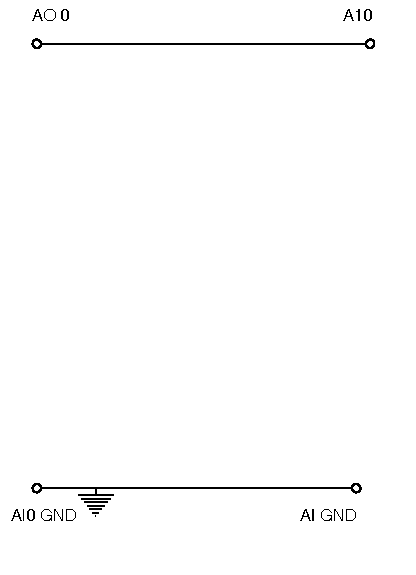
\includegraphics[scale=0.65]{/Users/ohyamasan/Downloads/TMCIT-Report/EE_Measurement/fig/5-volt.pdf}
\caption{変電圧計測回路}
\label{fig:5-volt}
\end{figure}

\subsubsection{出力電圧表示値と計測電圧値を配列・文字列で表示}
\begin{enumerate}[a)]
	\item 上記のプログラムの全てのプログラムを``For ループ''で囲むように配置.コネクタ``N''に定数を作成し,5を代入.
	\item ``Analog Output''の左コネクタ(A/AO 0 pin2)をカウンタ変数``i''に接続.(制御器``AO0''との接続は予め解除しておく)
	\item ``配列連結追加''ブロックを追加し,その出力コネクタから伸ばしたワイヤーを``For ループ枠''に繋げ,表示器を新規作成.
	\item 作成したプログラムを実行し,``配列''に表示される電圧値を予想される値と比較した.
	\item ブロックダイアグラムに``遅延時間''を追加し,制御器を追加.``遅延時間''は0.05\,秒に設定.
	\item ``AnalogOutput''の``error out''と``遅延時間''の``エラー入力'',``遅延時間''の``エラー出力''と``AnalogOutput''の``error in''を接続.
	\item ``遅延時間''ブロックの追加による``配列''に表示される値の変化を確認した.
	\item 遅延時間を,0\,秒, 0.005\,秒, 0.050\,秒, 0.500\,秒に変え,それぞれの場合で入力値を変更し,表示値との比較を行った.(3.5.2のように2回目以降は入力値と出力値がほぼ一致した)
	\item 以降の手順は3.3.3および3.3.4を参照し,文字列を表示させる.
\end{enumerate}


\subsection{実習2-2 課題実験}
\begin{enumerate}[a)]
	\item 0\,\rm{V}から5\,\rm{V}まで0.5\,\rm{V}刻みで出力電圧を変え,出力電圧値を計測.
	\item ``Analog Output''に入力した値・``Analog Input''から取得した値をカウンタ変数``i'', ``Analog Output''表示値・``Analog Input''表示値を表示.
	\item ``出力電圧表示値''と``計測電圧表示値''との差を表示.
	\item 上で導出した差から二乗平均平方根誤差(Root Mean Squared Error, RMSE)をExcelを用いて求めた.
\end{enumerate}


\subsection{実習3}
\subsubsection{固定抵抗の電圧電流特性}
\begin{enumerate}[a)]
	\item \wfig{mesure-vl}のように回路を構築.
	\item V, $V_{U}$, $R_{0}$を用いて電圧,電流を計測し電圧-電流特性を計測する.なお測定対象素子は,1\,k\rm{$\Omega$}.$R_{0}$の抵抗値変化は,100\,\rm{$\Omega$},1\,k\rm{$\Omega$},10\,k\rm{$\Omega$},100\,k\rm{$\Omega$}である.
\end{enumerate}

\begin{figure}[h]
\centering
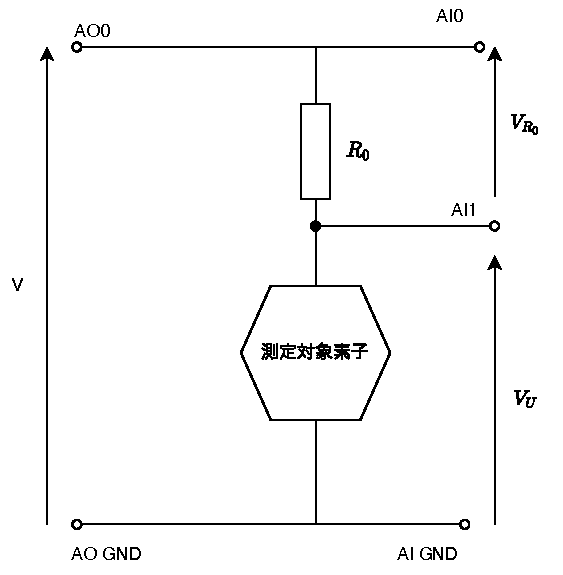
\includegraphics[scale=0.75]{/Users/ohyamasan/Downloads/TMCIT-Report/EE_Measurement/fig/mesure-vl.pdf}
\caption{電圧電流特性計測回路}
\label{fig:mesure-vl}
\end{figure}


\subsubsection{可変抵抗(ポテンショメータ)の電圧電流特性}
\begin{enumerate}[a)]
	\item \wfig{mesure-vl}において,測定素子を可変抵抗に変更.
	\item \wfig{poten}を参考にして,可変抵抗の端子間を1-2としてつまみ位置をA, B, C (くぼみが向いている向きがA, B, Cとなるように.すなわち,図ではAの状態である)にして,それぞれの電圧を計測した.なお,プログラムは上で作成したものをそのまま利用した.
	\item 可変抵抗の端子間を2-3, 3-1間でも同様に測定した.
	\item ただし,$R_{0}$は測定データを基に適切なものを選択した.
\end{enumerate}

\begin{figure}[h]
\centering
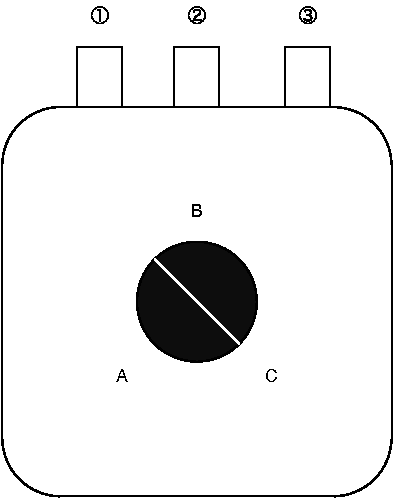
\includegraphics[scale=0.6]{/Users/ohyamasan/Downloads/TMCIT-Report/EE_Measurement/fig/potencial.pdf}
\caption{ポテンショメータ}
\label{fig:poten}
\end{figure}

\subsubsection{CdSセンサの電圧電流特性}
\begin{enumerate}[a)]
	\item \wfig{mesure-vl}の測定素子をCdSセンサ(\wfig{CdS})に変更.
	\item 自然状態とスマホのライトをセンサ部分に照射する場合のそれぞれで,上と同様に測定を行った.
	\item ただし,$R_{0}$は測定データを基に適切なものを選択した.
\end{enumerate}

\begin{figure}[h]
\centering
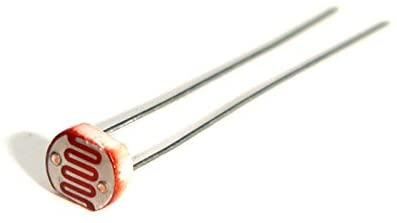
\includegraphics[scale=0.5]{/Users/ohyamasan/Downloads/TMCIT-Report/EE_Measurement/fig/31AbZ9saczL._AC_.jpg}
\caption{CdSセンサ\cite{cbs}}
\label{fig:CdS}
\end{figure}

\subsubsection{力センサの電圧電流特性}
\begin{enumerate}[a)]
	\item  \wfig{mesure-vl}の測定素子を力センサ(\wfig{power})に変更.
	\item 自然状態とセンサ部分(黒い枠で囲まれている円部分)を強く押し続けた状態のそれぞれで,上と同様に測定を行った.
	\item ただし,$R_{0}$は測定データを基に適切なものを選択した.
\end{enumerate}

\begin{figure}[h]
\centering
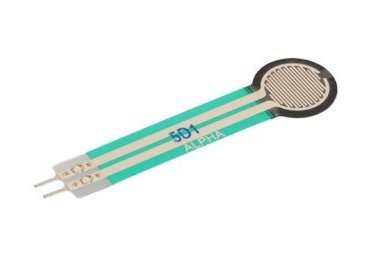
\includegraphics[scale=0.5]{/Users/ohyamasan/Downloads/TMCIT-Report/EE_Measurement/fig/31Gu87ucreL.jpg}
\caption{力センサ\cite{power}}
\label{fig:power}
\end{figure}

\subsubsection{発光ダイオードの電圧電流特性}
\begin{enumerate}[a)]
	\item \wfig{mesure-vl}の測定素子をLEDに変更.
	\item 測定するLEDは発光色4種類(赤,青,白,緑)で行った.
	\item ただし,$R_{0}$は測定データを基に適切なものを選択した.
\end{enumerate}